\section{Application I}
This section will demonstrate the size optimization of a cantilever beam consisting of five different parts.

\sidenote{
    
\qrcode[height=1in]{https://github.com/btayfur/structural-optimization/blob/main/Code/Examples/Exmp6/}}

\subsection{Problem Definition}
In this application, an optimization problem aiming to minimize the weight of a 3-meter-long cantilever beam divided into 5 equal parts will be addressed. The details of the problem are as follows:

\begin{itemize}
    \item A 3-meter-long cantilever beam divided into 5 equal parts
    \item Each part has a hollow circular cross-section with two design parameters:
    \begin{itemize}
        \item $r_{outer}$: Outer radius
        \item $r_{inner}$: Inner radius
    \end{itemize}
    \item Material: S270 steel (E = 210 GPa, $\sigma_y$ = 270 MPa)
    \item A force F = 500 kN is applied perpendicular to the free end of the beam
    \item Objective: Minimize the weight of the beam
\end{itemize}

\subsubsection{Constraints}
\begin{enumerate}
    \item A maximum displacement of 2 cm is allowed at the free end of the beam
    \item For each part, the outer radius must be greater than the inner radius
    \item The inner radius of the previous part must be smaller than the outer radius of the next part (weldability condition)
    \item The yield stress of S270 steel (270 MPa) must not be exceeded
\end{enumerate}

\subsection{Structural Analysis}
The finite element method has been used for displacement and stress analysis of the cantilever beam:

\begin{itemize}
    \item Each beam part is modeled as an Euler-Bernoulli beam element
    \item Each node has 2 degrees of freedom (displacement and rotation)
    \item Global stiffness matrix is created to calculate displacements
    \item Stresses are calculated using bending moment and section properties
\end{itemize}

\subsubsection{Stiffness Matrix Formation}
The stiffness matrix for the beam element is formed as follows:

\begin{equation}
k_e = \begin{bmatrix}
\frac{12EI}{l^3} & \frac{6EI}{l^2} & -\frac{12EI}{l^3} & \frac{6EI}{l^2} \\
\frac{6EI}{l^2} & \frac{4EI}{l} & -\frac{6EI}{l^2} & \frac{2EI}{l} \\
-\frac{12EI}{l^3} & -\frac{6EI}{l^2} & \frac{12EI}{l^3} & -\frac{6EI}{l^2} \\
\frac{6EI}{l^2} & \frac{2EI}{l} & -\frac{6EI}{l^2} & \frac{4EI}{l}
\end{bmatrix}
\end{equation}

Where:
\begin{itemize}
    \item $E$: Young's modulus
    \item $I$: Moment of inertia
    \item $l$: Element length
\end{itemize}

Moment of inertia for hollow circular cross-section:
\begin{equation}
I = \frac{\pi}{4}(r_{outer}^4 - r_{inner}^4)
\end{equation}

\subsubsection{Boundary Conditions and Solution}
The left end of the cantilever beam is fixed, therefore the degrees of freedom at the first node are zero. The force applied to the right end is added to the global force vector. The displacement vector is solved using the reduced stiffness matrix and force vector:

\begin{equation}
\mathbf{K_{reduced}} \cdot \mathbf{u} = \mathbf{F}
\end{equation}

\subsection{Optimization Approach}
The Simulated Annealing algorithm has been used for optimization:

\begin{itemize}
    \item Random search strategy to avoid local optima
    \item Adaptive step size for effective exploration of solution space
    \item Slow cooling of process temperature to find better solutions
    \item Effective control of constraints to ensure physically feasible solutions
\end{itemize}

\subsubsection{Objective Function}
The objective function is the total weight of the beam:

\begin{equation}
W = \rho \sum_{i=1}^{5} A_i \cdot l_i
\end{equation}

Where:
\begin{itemize}
    \item $\rho$: Material density
    \item $A_i$: Cross-sectional area of each part ($A_i = \pi(r_{outer,i}^2 - r_{inner,i}^2)$)
    \item $l_i$: Length of each part
\end{itemize}

\subsubsection{Constraint Functions}
Four constraint functions are used in the optimization process:

\begin{enumerate}
    \item Displacement constraint: $u_{max} \leq 0.02$ m
    \item Radius constraint: $r_{outer,i} > r_{inner,i}$ (for each part)
    \item Weldability constraint: $r_{inner,i} < r_{outer,i+1}$ (for adjacent parts)
    \item Stress constraint: $\sigma_{max} \leq \sigma_{yield}$
\end{enumerate}

\subsection{Optimization Results}
The optimization resulted in a lighter beam design compared to the initial design:

\begin{itemize}
    \item Initial design weight: $\sim$1924 kg
    \item Optimized design weight: $\sim$939 kg (51\% reduction)
\end{itemize}

\begin{figure}[H]
    \centering
    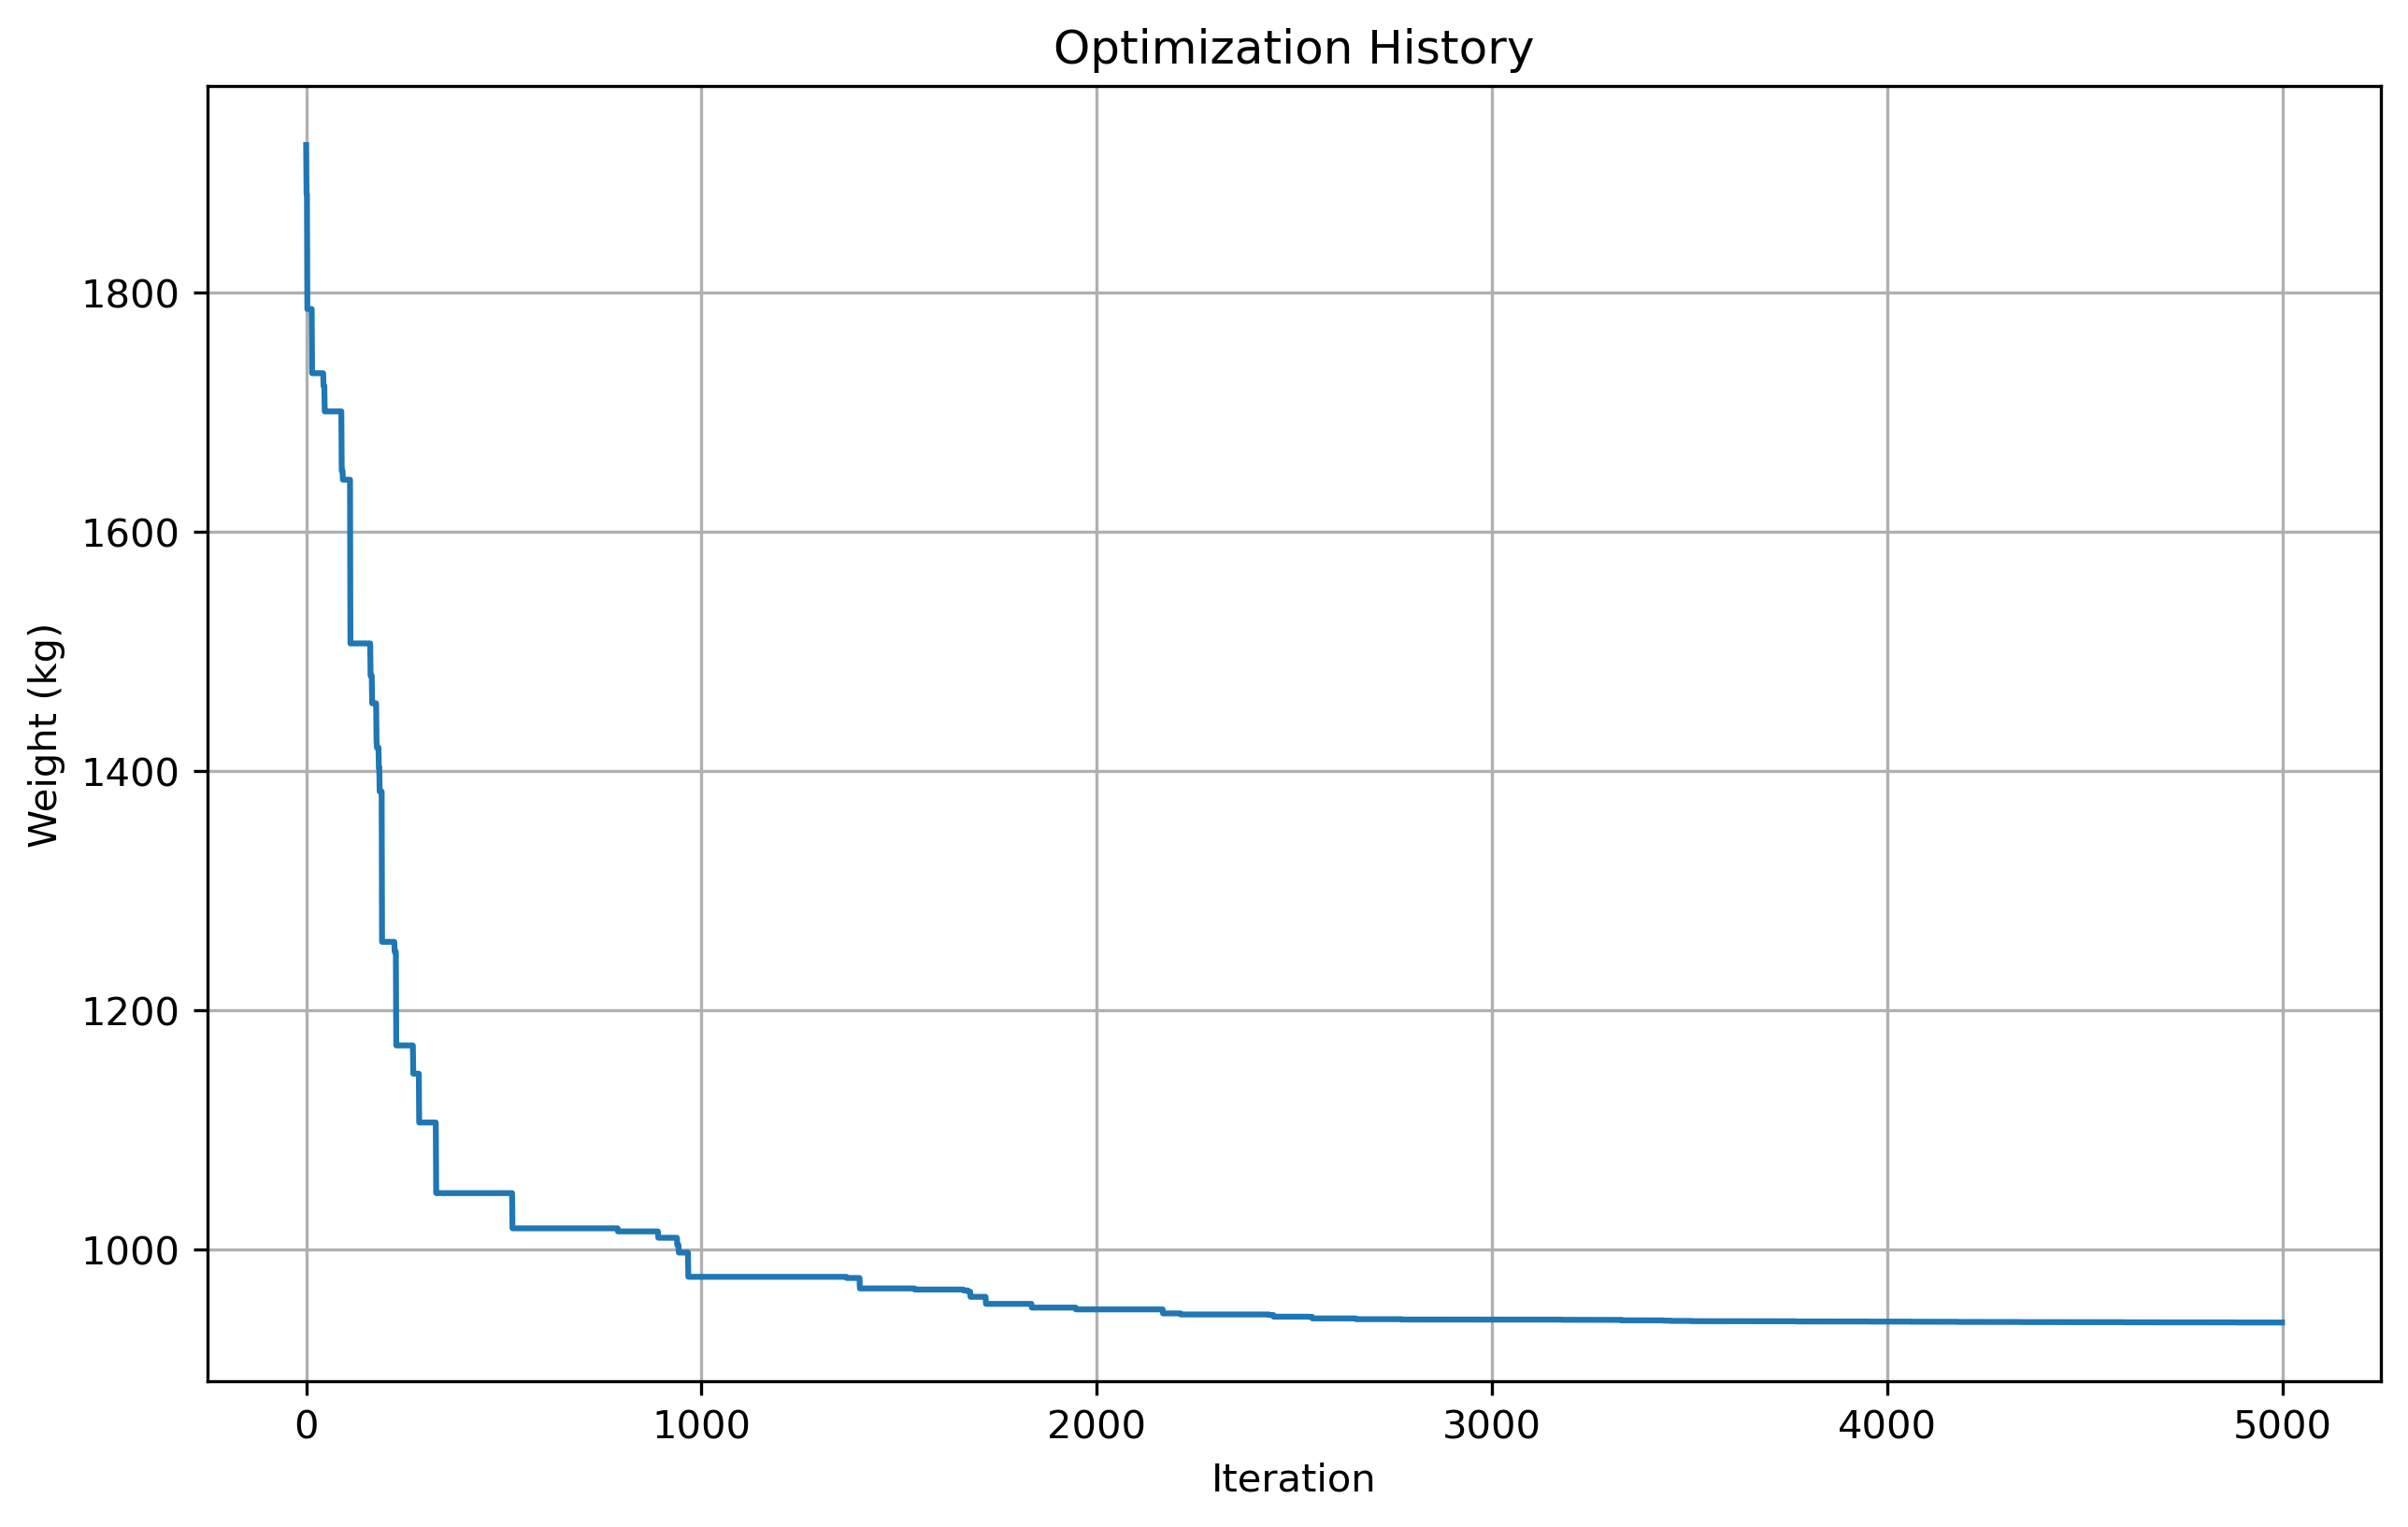
\includegraphics[width=1\textwidth]{weeks_new/imgs/optimization_history.png}
    \caption{Weight Tracking Graph}
    \label{fig:optimization_history}
\end{figure}

\subsubsection{Optimized Radii (cm)}
\begin{center}
\begin{tabular}{|c|c|c|}
\hline
Part & Outer Radius ($r_{outer}$) & Inner Radius ($r_{inner}$) \\
\hline
1 & 20.37 & 14.36 \\
2 & 20.05 & 15.81 \\
3 & 15.82 & 9.04 \\
4 & 16.00 & 13.33 \\
5 & 14.26 & 13.30 \\
\hline
\end{tabular}
\end{center}

In the optimized design:
\begin{itemize}
    \item The displacement at the end point is 0.12 cm (maximum allowed 2 cm)
    \item The stress constraint is active (0.00 MPa margin)
    \item The cross-section dimensions satisfy the weldability condition
\end{itemize}

\subsubsection{Optimized Beam Design}
The geometry of the optimized beam shows that the cross-section dimensions decrease from the support point (left side) towards the free end. This is consistent with the bending moment being maximum at the support and decreasing towards the free end.
\begin{figure}[H]
    \centering
    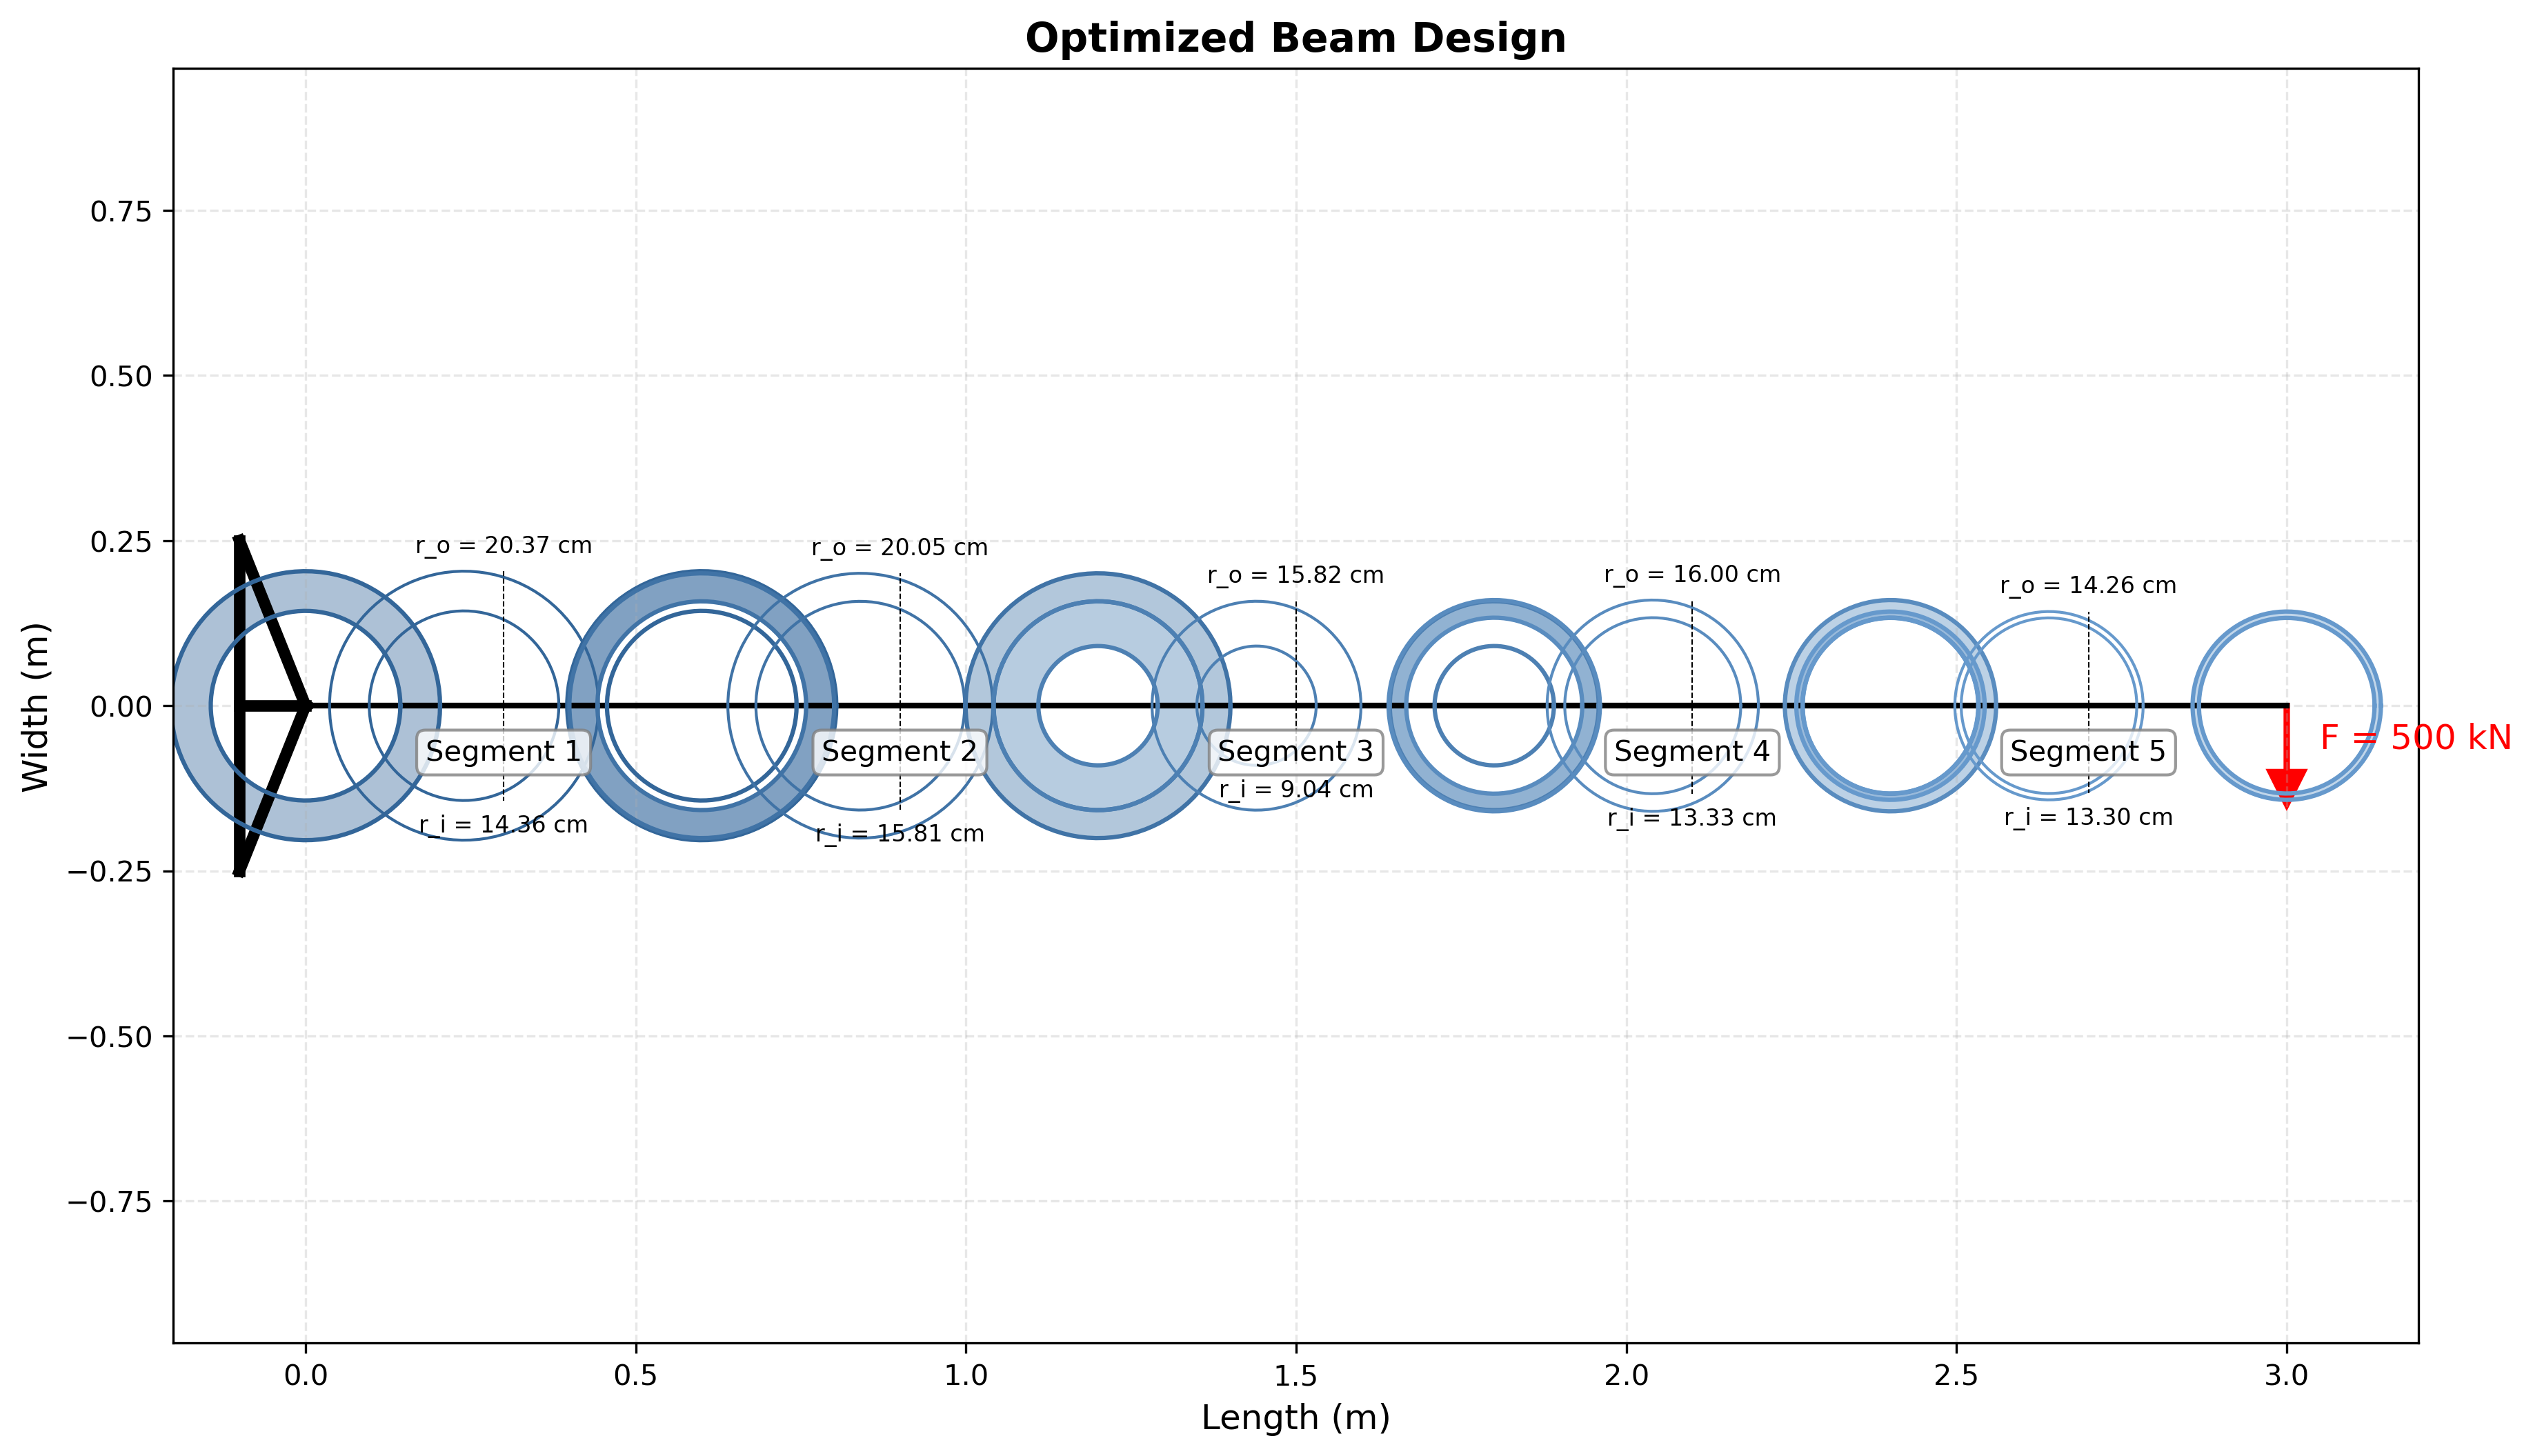
\includegraphics[width=1\textwidth]{weeks_new/imgs/optimized_beam.png}
    \caption{Optimized Beam Design}
    \label{fig:optimized_beam}
\end{figure}

\subsubsection{Deformation Shape}
The deformation shape of the cantilever beam under load has a maximum displacement of 2 cm at the free end. The displacement values at each node are also shown.

\begin{figure}[H]
    \centering
    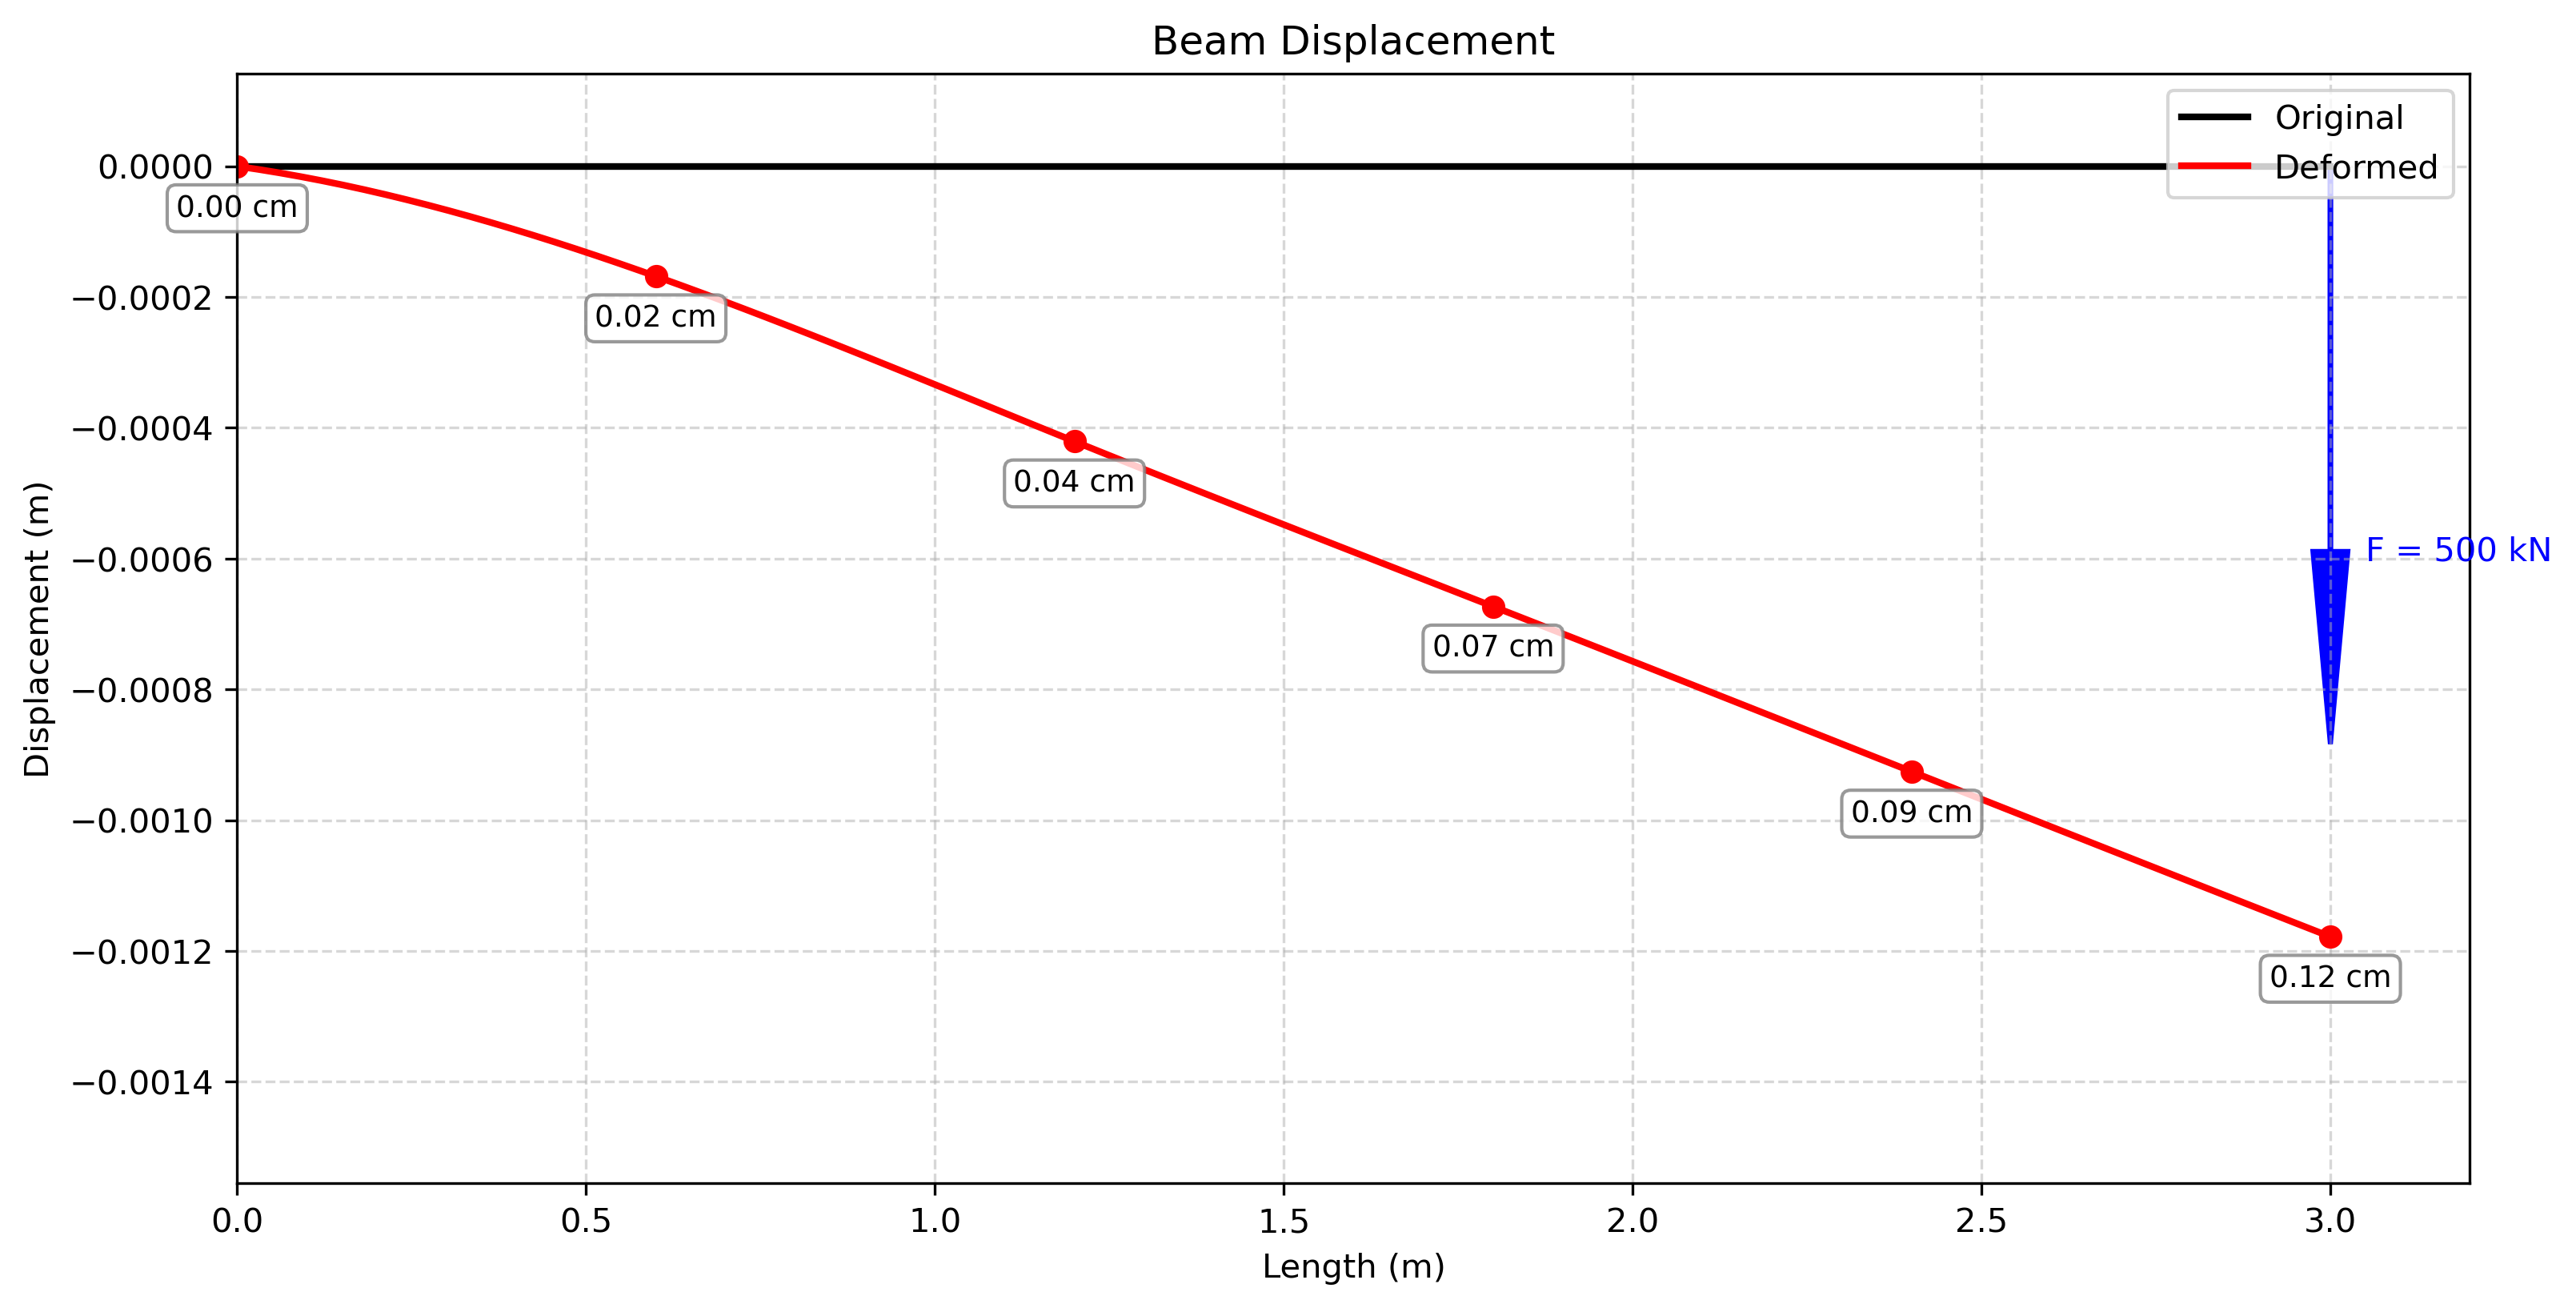
\includegraphics[width=1\textwidth]{weeks_new/imgs/deformed_beam.png}
    \caption{Deformation Shape}
    \label{fig:deformed_beam}
\end{figure}

\subsubsection{Constraint Utilization Ratios}
Graphs have been created showing how much each constraint is utilized in the optimized design:

\begin{itemize}
    \item \textbf{Displacement Constraint:} Maximum displacement limit is fully utilized (100\%)
    \item \textbf{Stress Constraint:} Yield stress utilization ratio for each segment
    \item \textbf{Radius Ratio:} Ratio of inner radius to outer radius
    \item \textbf{Weldability:} Utilization ratio of the welding condition between adjacent segments
\end{itemize}

\begin{figure}[H]
    \centering
    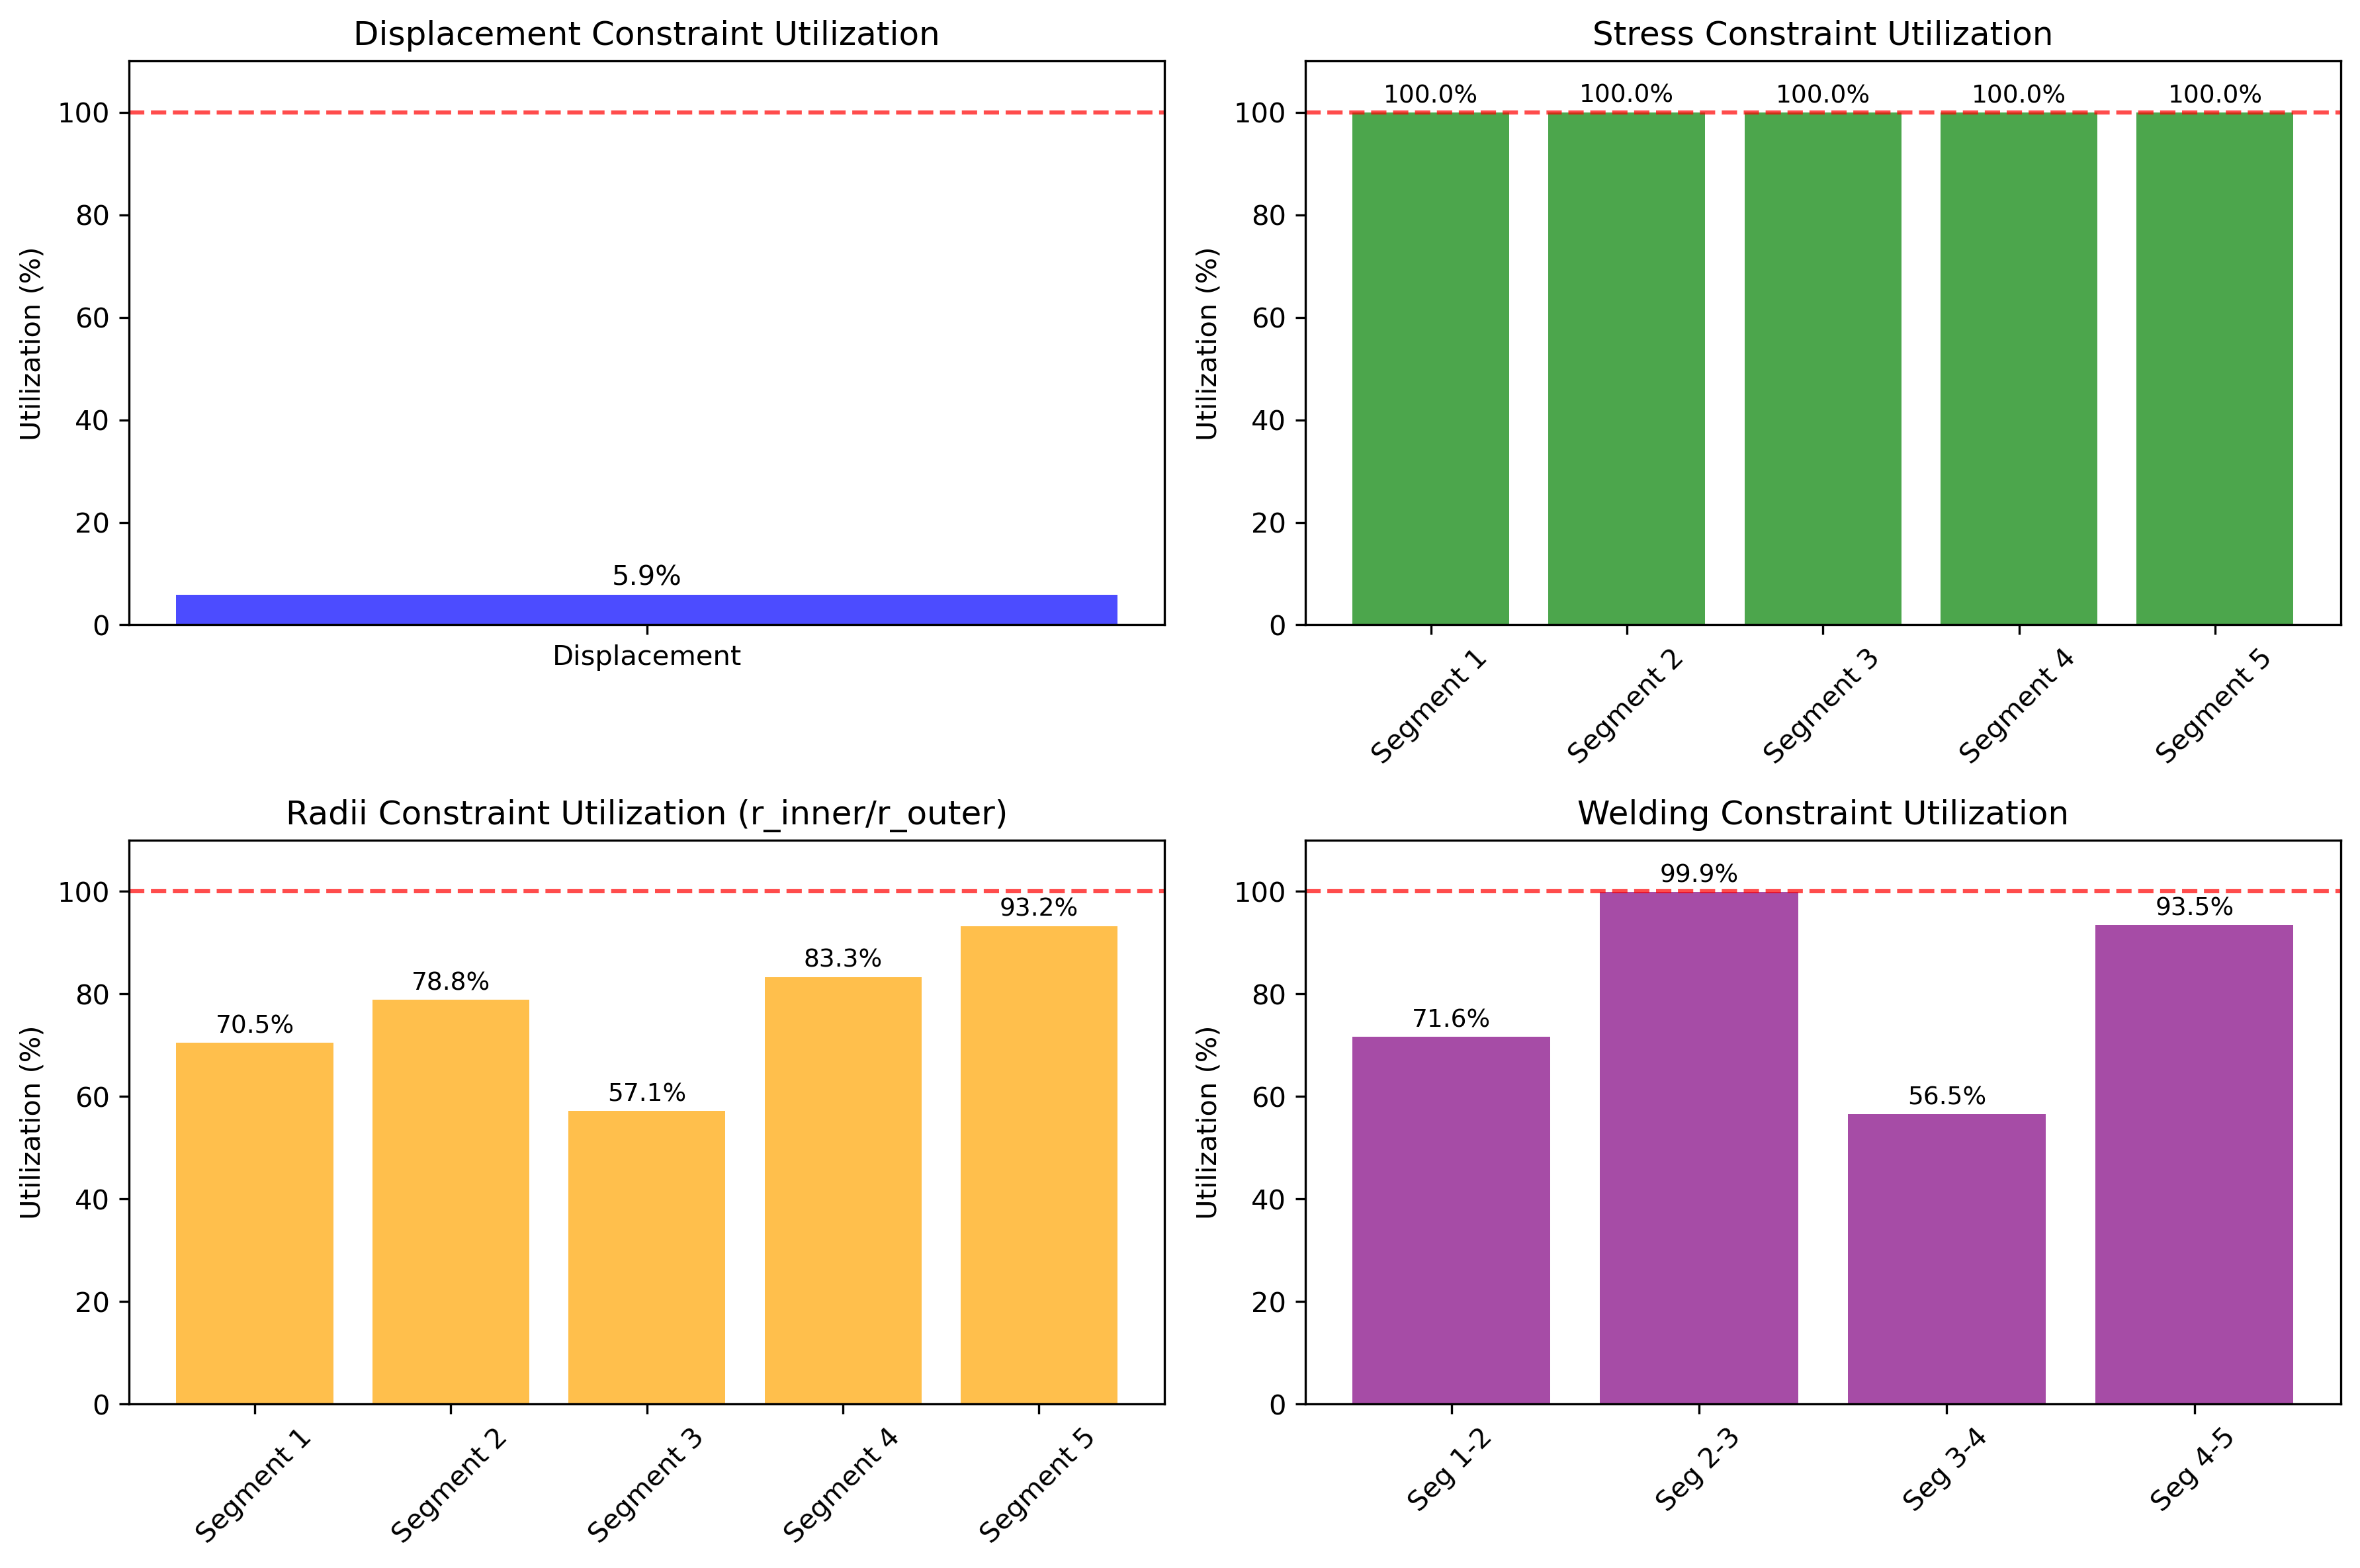
\includegraphics[width=1\textwidth]{weeks_new/imgs/constraint_utilization.png}
    \caption{Constraint Capacity Utilization Ratios}
    \label{fig:constraint_utilization}
\end{figure}

As can be seen from the graphs, the displacement constraint is active in the optimal design (fully utilized). This indicates that the optimized design has reached the limit in terms of weight minimization.

\subsection{Conclusion and Evaluation}
In this application, the optimal design of a cantilever beam for minimum weight under constraints has been obtained using the Simulated Annealing optimization algorithm. The results show that a structure 51\% lighter than the initial design has been achieved.

In the optimized design, it is observed that particularly the stress constraint is fully utilized (active). This is an expected theoretical result in weight minimization problems, as typically at least one constraint is expected to be active.

The gradual decrease in beam geometry from the support point towards the free end is also an expected structural result. Since the bending moment is maximum at the support point, larger cross-sections have formed in this region. 